%% LaTeX-Beamer template for KIT design
%% by Erik Burger, Christian Hammer
%% title picture by Klaus Krogmann
%%
%% version 2.1
%%
%% mostly compatible to KIT corporate design v2.0
%% http://intranet.kit.edu/gestaltungsrichtlinien.php
%%
%% Problems, bugs and comments to
%% burger@kit.edu

\documentclass[14pt,t]{beamer}

\beamertemplatenavigationsymbolsempty{}

\usepackage[ruled,linesnumbered]{algorithm2e}
\usepackage{ccicons}
\usepackage{csquotes}
\usepackage{nth}
\usepackage{relsize}
\usepackage{siunitx}

\usefonttheme{professionalfonts}
\usepackage{fontspec}
\usepackage{unicode-math}
\defaultfontfeatures{
    Ligatures=TeX
}
\setmathfont[Scale=0.98]{xits-math.otf}
%\defaultfontfeatures{Ligatures=Rare}
\setmainfont{Source Sans Pro}[Scale = 0.9]
\setsansfont{Source Sans Pro}[Scale = 0.9]
\setmonofont{VeraMono}[
    Path           = /usr/share/fonts/TTF/,
    Extension      = .ttf,
    BoldFont       = VeraMoBd,
    ItalicFont     = VeraMoIt,
    BoldItalicFont = VeraMoBI,
    Scale          = 0.78
]
\usepackage[activate={true,nocompatibility},final]{microtype}

%% SLIDE FORMAT

% use 'beamerthemekit' for standard 4:3 ratio
% for widescreen slides (16:9), use 'beamerthemekitwide'

\usepackage{templates/beamerthemekit}
% \usepackage{templates/beamerthemekitwide}

% Disable shading between block title and block content
\makeatletter
\pgfdeclareverticalshading[lower.bg,upper.bg]{bmb@transition}{200cm}{color(0pt)=(lower.bg); color(4pt)=(lower.bg); color(4pt)=(upper.bg)}
\makeatother

% braces for items
% http://tex.stackexchange.com/a/151958/25791
\usepackage{tikz}
\usetikzlibrary{calc,decorations.pathreplacing}
\newcounter{itemnum}
\newcommand{\nt}[2][0pt]{%
    \stepcounter{itemnum}%
    \if###2##%
    \else
        #2%
        \thinspace
    \fi
    \tikz[overlay,remember picture,baseline=(\theitemnum.base),xshift=#1]\node (\theitemnum){};%
}
\newcommand{\makebrace}[4]{%
    \begin{tikzpicture}[overlay, remember picture]
        \draw [decoration={brace,amplitude=0.5em},decorate]
        let \p1=(#2), \p2=(#3) in
        (#1, {\y1+1.75ex}) --
            node[right=0.6em] {#4} (#1, {\y2-0.5ex});
    \end{tikzpicture}%
}
\newenvironment{benumerate}{%
    \begin{enumerate}
}{%
    \end{enumerate}
    \setcounter{itemnum}{0}%
}
\newenvironment{bitemize}{%
    \begin{itemize}
}{%
    \end{itemize}
    \setcounter{itemnum}{0}%
}

% ball looks horrible
\defbeamertemplate{section in toc}{circle2}
{\leavevmode\leftskip=2ex%
  \llap{%
    \usebeamerfont*{section number projected}%
    \usebeamercolor{section number projected}%
    \begin{pgfpicture}{-1ex}{-0.7ex}{1ex}{2ex}
      \color{bg}
      \pgfpathcircle{\pgfpoint{.075ex}{.55ex}}{1.4ex}
      \pgfusepath{fill}
      \pgftext[base]{\color{fg}\textsmaller{\inserttocsectionnumber}}
    \end{pgfpicture}\kern1.25ex%
  }%
  \inserttocsection\par}
\setbeamertemplate{enumerate items}{%
  \usebeamerfont*{item projected}%
  \usebeamercolor{item projected}%
  \begin{pgfpicture}{-1ex}{-0.7ex}{1ex}{2ex}
    \color{bg}
    \pgfpathcircle{\pgfpoint{.075ex}{.55ex}}{1.4ex}
    \pgfusepath{fill}
    \pgftext[base]{\color{fg}\textsmaller{\insertenumlabel}}
  \end{pgfpicture}%
}
\setbeamertemplate{section in toc}[circle2]

% section pages
\setbeamerfont{section title}{family=\sffamily,series=\bfseries,size=\LARGE}
\setbeamertemplate{section page}
{
  \begin{centering}
    \begin{beamercolorbox}[sep=4pt,center]{part title}
      \usebeamerfont{section title}\insertsection\par
    \end{beamercolorbox}
  \end{centering}
}
\AtBeginSection{\frame[c]{\sectionpage}}

%% TITLE PICTURE

% if a custom picture is to be used on the title page, copy it into the 'logos'
% directory, in the line below, replace 'mypicture' with the
% filename (without extension) and uncomment the following line
% (picture proportions: 63 : 20 for standard, 169 : 40 for wide
% *.eps format if you use latex+dvips+ps2pdf,
% *.jpg/*.png/*.pdf if you use pdflatex)

\titleimage{cover}

%% TITLE LOGO

% for a custom logo on the front page, copy your file into the 'logos'
% directory, insert the filename in the line below and uncomment it

\titlelogo{empty}

% (*.eps format if you use latex+dvips+ps2pdf,
% *.jpg/*.png/*.pdf if you use pdflatex)

%% TikZ INTEGRATION

% use these packages for PCM symbols and UML classes
% \usepackage{templates/tikzkit}
% \usepackage{templates/tikzuml}

% the presentation starts here

\title[CASINO TIMES]{\textsmaller{\textsmaller{Compression and Similarity Indexing for Time Series}}}
\subtitle{Master's Thesis}
\author{Marco Neumann}
\date{\nth{19} of August 2016}

\institute{Chair Prof.\ Böhm}

% Bibliography

\usepackage[citestyle=authoryear,bibstyle=numeric,hyperref,backend=biber]{biblatex}
\addbibresource{../tex/thesis.bib}
\bibhang1em
\renewcommand*{\bibfont}{\tiny}
\setbeamertemplate{bibliography item}[text]

\begin{document}

% change the following line to "ngerman" for German style date and logos
\selectlanguage{english}

%title page
\begin{frame}
\titlepage
\end{frame}

%table of contents
\begin{frame}{Outline}
\tableofcontents
\end{frame}

\section{Google $n$-gram data}
\stepcounter{subsection}
\begin{frame}[c]{Public Data Set}
    \begin{center}
        \includegraphics[width = \textwidth]{img/ngram-website}
    \end{center}
\end{frame}
\begin{frame}{Information Provided by the Data Set}
    Similarities $=$ hints for common cause

    \vfill{}

    \begin{alertblock}{Warning}
        similarity $\neq$ causality
    \end{alertblock}
\end{frame}
\begin{frame}{Current problems}
    \begin{itemize}
        \item \enquote{similarity} is not precisely defined
        \item manual analysis
            \begin{itemize}
                \item slow
                \item confirmation bias
                \item choosing possible candidates is subject to frame
            \end{itemize}
        \item data is \enquote{big}\footnote{for interactive analysis}
    \end{itemize}
\end{frame}
\begin{frame}{Goals}
    \begin{itemize}
        \item exact description of \enquote{similarity}
        \item allowing of interactive nearest neighbor queries
            \begin{itemize}
                \item design \& evaluation of baseline
                \item design \& evaluation of an own approach
            \end{itemize}
    \end{itemize}
\end{frame}

\section{Clean-up}
\stepcounter{subsection}
\begin{frame}{Steps}
    \begin{enumerate}
        \item string filtering:
            \begin{itemize}
                \item numbers
                \item word classes
            \end{itemize}
        \item string normalization:
            \begin{itemize}
                \item NFKC Unicode normalization
                \item lowercase
            \end{itemize}
        \item word normalization:
            \begin{itemize}
                \item stemming
                \item lemmatisation
            \end{itemize}
        \item pruning:
            \begin{itemize}
                \item rare words
                \item OCR errors
                \item only last \num{256} years
            \end{itemize}
    \end{enumerate}
\end{frame}
\begin{frame}[c]{Results}
    \begin{center}
        \includegraphics[width = \textwidth]{img/clean-up}
    \end{center}
    \vspace{\baselineskip}
    $1$-grams: $\approx$\num{800000}

    $2$-grams: $\approx$\num{6400000}
\end{frame}

\section{Similarity}
\stepcounter{subsection}
\begin{frame}[c]{Input Data}
    \begin{center}
        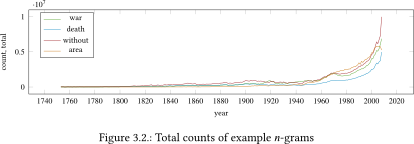
\includegraphics[width = \textwidth]{img/example-noop}
    \end{center}
\end{frame}
\begin{frame}[c]{Normalization}
    \begin{center}
        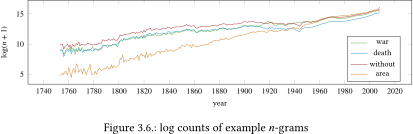
\includegraphics[width = \textwidth]{img/example-log}
    \end{center}
\end{frame}
\begin{frame}[c]{(Smooth) Gradients}
    \begin{center}
        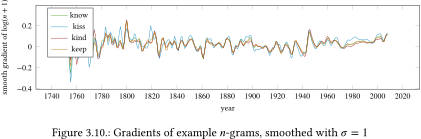
\includegraphics[width = \textwidth]{img/example-gradient-smooth}
    \end{center}
\end{frame}
\begin{frame}{DTW}
    Similar structure, but sometimes slightly off

    \vspace{0.5\baselineskip}

    $\Rightarrow$ use Dynamic Time Warping (DTW)

    (limited by a Sakoe-Chiba Band of radius $r$)

    \begin{center}
        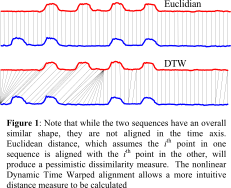
\includegraphics[width = 0.4\textwidth]{img/bib-dtw}
    \end{center}

    \textsmaller[4]{
        VLDB, 2002, Exact Indexing of Dynamic Time Warping;

        \vspace{-\baselineskip}

        copying is by permission of the Very Large Data Base Endowment.
    }
\end{frame}
\begin{frame}{Final Order}
    \begin{benumerate}
        \item \nt{$\log(x + 1)$}
        \item \nt{Gauss-smoothing\\using $\sigma$}
        \item \nt{gradient calculation}
        \item \nt{}DTW with warping\\radius of $r$\nt{}
    \end{benumerate}
    \makebrace{150pt}{1}{3}{\textsmaller{\textit{pre-calculation}}}\makebrace{150pt}{4}{5}{\textsmaller{\textit{on demand}}}
\end{frame}
\begin{frame}[c]{Sanity Check}
    \begin{center}
        
\includegraphics[width = \textwidth]{img/table-nn-good}
    \end{center}
\end{frame}
\begin{frame}[c]{Examples of Philosophic Institute}
    \begin{center}
        
\includegraphics[width = \textwidth]{img/table-nn-semigood}
    \end{center}
\end{frame}

\section{Baseline}
\stepcounter{subsection}
\begin{frame}[c]{R-tree-based index}
    \begin{center}
        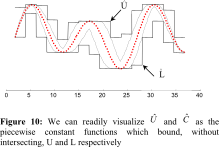
\includegraphics[width = 0.7\textwidth]{img/bib-lb_keogh}
    \end{center}

    \vspace{\baselineskip}

    \textsmaller[4]{
        VLDB, 2002, Exact Indexing of Dynamic Time Warping;

        \vspace{-\baselineskip}

        copying is by permission of the Very Large Data Base Endowment.
    }
\end{frame}
\begin{frame}[c]{Index Inefficiency}
    \begin{center}
        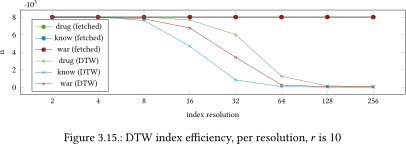
\includegraphics[width = \textwidth]{img/baseline}
    \end{center}
\end{frame}
\begin{frame}[c]{Performance}
    \begin{center}
        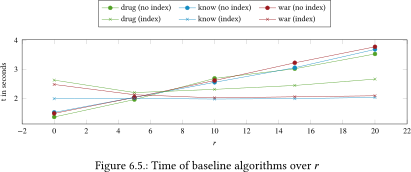
\includegraphics[width = \textwidth]{img/perf-baseline}
    \end{center}
\end{frame}

\section{CASINO TIMES}
\stepcounter{subsection}
\begin{frame}{Goals}
    \begin{itemize}
        \item primary:
            \begin{itemize}
                \item speed up nn queries using an index
                \item compress data
            \end{itemize}
        \item secondary:
            \begin{itemize}
                \item enable subrange queries w/o re-indexing
                \item slow pre-processing, fast search
                \item use normal hardware
            \end{itemize}
    \end{itemize}
\end{frame}
\begin{frame}[c]{Wavelet decomposition}
    \begin{center}
        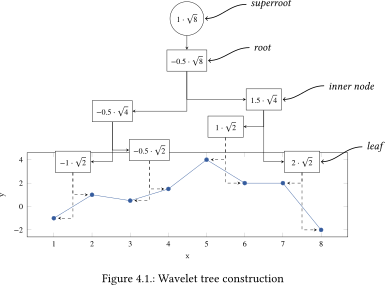
\includegraphics[width = 0.8\textwidth]{img/wavelet-tree}
    \end{center}
\end{frame}
\begin{frame}{Information Merging}
    \begin{itemize}
        \item search similar subtrees (of different time series)
        \item process one whole tree at the time
        \item node-by-node greedy method
        \item merge node if:
            \begin{itemize}
                \item same children
                \item difference of coefficients is small\\($=$ compression error is below threshold)
            \end{itemize}
    \end{itemize}
\end{frame}
\begin{frame}[c]{Example}
    \begin{center}
        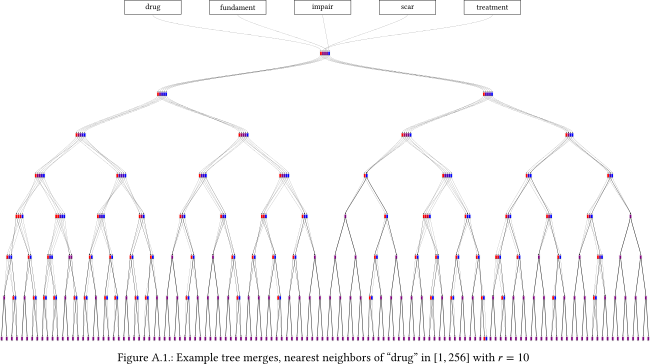
\includegraphics[width = \textwidth]{img/merge}
    \end{center}
\end{frame}
\begin{frame}[c]{Example (zoomed)}
    \begin{center}
        \includegraphics[width = 0.275\textwidth]{img/merge-zoom}
    \end{center}
\end{frame}
\begin{frame}[c]{Weakness}
    \begin{center}
        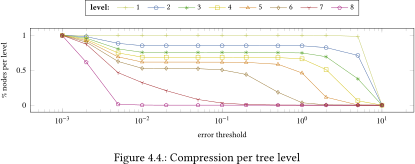
\includegraphics[width = \textwidth]{img/weakness}
    \end{center}
\end{frame}
\begin{frame}{Failed Improvements}
    \begin{itemize}
        \item merge entire subtrees (same index structure)
        \item merge entire subtrees (FLANN)
        \item random boosting
        \item DTW for leaves
        \item drop time constraint for leaves
        \item information / subtree pruning
        \item DB seeding
    \end{itemize}
\end{frame}

\section{Final Words}
\stepcounter{subsection}
\begin{frame}{Conclusion}
    \begin{itemize}
        \item foundation for future research\footnote{starting collaboration with Prof.\ Dr.\ Sanders}:
            \begin{itemize}
                \item definition of similarity
                \item fast baseline algorithm
            \end{itemize}
        \item knowledge about tree-like methods\\$\Rightarrow$ not promising
    \end{itemize}
\end{frame}
\begin{frame}{Possible Ideas}
    \begin{itemize}
        \item compression using:
            \begin{itemize}
                \item IEEE-half floating point
                \item non-IEEE data types (e.g.\ A-law and $\mu$-law)
            \end{itemize}
        \item general purpose compression of chunks\\(e.g.\ snappy, lz4, gzip, xz, brotli)
        \item static/dynamic downsampling
        \item locality-preserving hashing
        \item time series encoding using functions (e.g.\ cubic splines) $+$ patching
    \end{itemize}
\end{frame}

\begin{frame}{Thanks}
    \begin{itemize}
        \item Dr.-Ing.\ Martin Schäler
        \item Prof.\ Dr.-Ing.\ Klemens Böhm
        \item IPD IT team
        \item Philosophic Friends
        \item Miguel Angel Meza Martínez
    \end{itemize}
\end{frame}

\appendix
\beginbackup

\begin{frame}[allowframebreaks]{References}
    Title picture:\\
    \ccby{} 2013 \enquote{Casino Royale} by Rebecca Siegel\\
    \textsmaller{\url{https://www.flickr.com/photos/grongar/8704148177/}}
    \nocite{*}

    \vspace{\baselineskip}

    \printbibliography[heading=none]
\end{frame}
\begin{frame}[c]{Information Merging}
    \begin{center}
        \scalebox{.6}{
            \begin{algorithm}[H]
                \KwData{Trees $T$}
                \KwData{Error threshold $\epsilon$}

                \SetKwFunction{AddToDB}{addToDB}
                \SetKwFunction{ExecuteMerge}{executeMerge}
                \SetKwFunction{HasUntriedPossibleMerge}{hasUntriedPossibleMerge}
                \SetKwFunction{MaxErrIncrease}{maxErrIncrease}
                \SetKwFunction{MarkTried}{markTried}
                \SetKwFunction{PickCheapestMerge}{pickCheapestMerge}
                \SetKwFunction{RealErrIncrease}{realErrIncrease}
                \SetKwFunction{Shuffled}{shuffled}

                \Begin{
                    \For{$t$ $\in$ \Shuffled{$T$}}{
                        $e \leftarrow 0$\;
                        \While{\HasUntriedPossibleMerge{$t$}}{
                            $t \leftarrow \PickCheapestMerge{$t$}$\;
                            \If{$e$ $+$ \MaxErrIncrease{$m$} $\leq$ $\epsilon$}{
                                \ExecuteMerge{$m$}\;
                                $e \leftarrow e + \RealErrIncrease{$m$}$\;
                            }
                            \MarkTried{$t$}\;
                        }
                        \AddToDB{$t$}\;
                    }
                }

                \caption{runCompression}
            \end{algorithm}
        }
    \end{center}
\end{frame}
\begin{frame}[c]{Compression Distortion}
    \begin{center}
        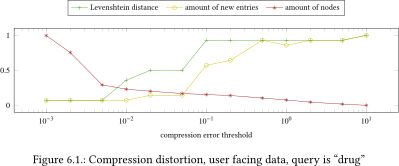
\includegraphics[width = \textwidth]{img/backup-distortion1}
    \end{center}
\end{frame}
\begin{frame}[c]{Compression Distortion}
    \begin{center}
        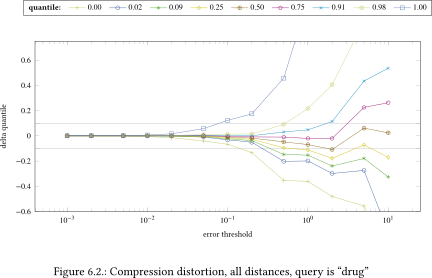
\includegraphics[width = \textwidth]{img/backup-distortion2}
    \end{center}
\end{frame}
\begin{frame}[c]{Tracer Quality}
    \begin{center}
        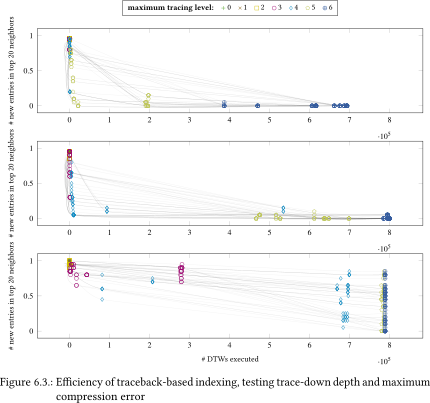
\includegraphics[width = 0.6\textwidth]{img/backup-tracer}
    \end{center}
\end{frame}
\begin{frame}[c]{Tracer Performance}
    \begin{center}
        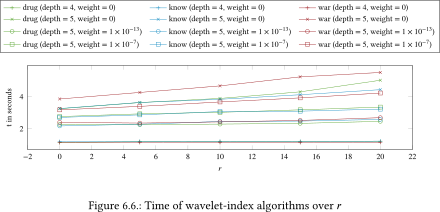
\includegraphics[width = \textwidth]{img/backup-perf-tracer}
    \end{center}
\end{frame}

\backupend

\end{document}
